\chapter{Interferenza di intersimbolo} 

\begin{figure}[h]
    \centering
    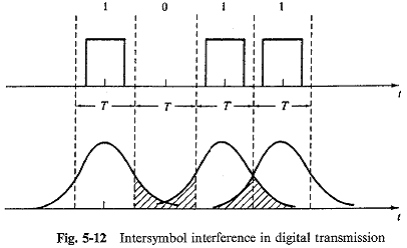
\includegraphics[scale = 1]{DigitalModulation_clip_image114.jpg}
\end{figure}  

\newpage 

\section{Da impulsi rettangolari alle forme d'onda reali}

Nell'accezione comune, le forme d'onda utilizzate in una trasmissione numerica hanno durata finita; 
in particolare, è frequente il caso in cui si utilizzino impulsi rettangolari di durata uguale o minore di un intervallo caratteristico, denominato tempo di simbolo. \newline 

\begin{figure}[h]
    \centering
    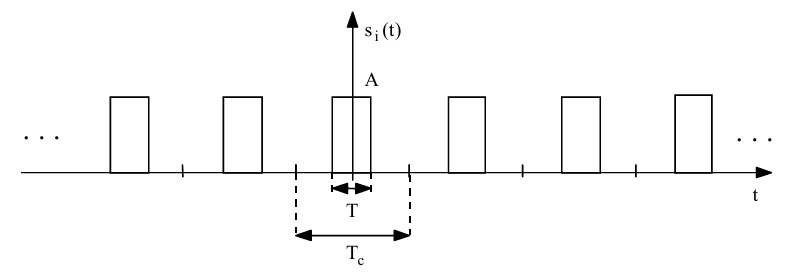
\includegraphics[scale = 0.8]{Impulsi rettangolari.PNG}
\end{figure}  

La trasmissione di un segnale numerico con queste caratteristice avrebbe, a rigore, bisogno di una banda infinita perchè ha fronti 
d'onda a pendenza elevata, nel caso di impulsi rettangolari la transizione è immediata, quindi banda illimitata. \newline 

Quando un segnale numerico si trova a transitare attraverso un filtro, ad esempio un canale di trasmissione, esso verrà inevitabilmente distorto. \newline 

Il segnale rettangolare visto in precedenza, dopo il passaggio ad un filtro, si può presentare come segue: 

\begin{figure}[h]
    \centering
    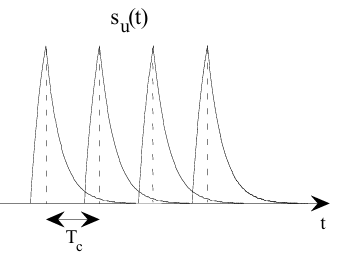
\includegraphics[scale = 0.8]{Impulsi rettangolari dopo un filtro.PNG}
\end{figure} 

Confrontando lo stesso segnale, prima e dopo il filtro, notiamo che gli impulsi binari, che sono ben distinti nel segnale di ingresso $s_i (t)$ rislutano sovrapposti nel segnale di uscita $s_u (t)$. \newline 

Trattandosi di un fenomeno (indesiderato) di interazione tra simboli, si è soliti parlare di inteferenza intersimbolica (in inglese ISI: InterSymbol Interference). \newline 

I simboli interferenti possono riferirsi allo stesso (e unico) segnale, o, nel caso delle comunicazioni, il mezzo trasmissivo è condiviso tra più utenti a divisione di tempo, 
in cui si usa lo stesso mezzo trasmissivo tra sorgente-destinazioni: in questo casa ci saranno degli effetti di mutuo disturbo tra le diverse comunicazioni. \newline 

\newpage 

\section{Diagramma ad occhio} 

Uno strumento molto utile nel capire l'effetto dell'ISI in un segnale è quello del diagramma ad occhio. \newline 

Un esempio di diagramma ad occhio: 

\begin{figure}[h]
    \centering
    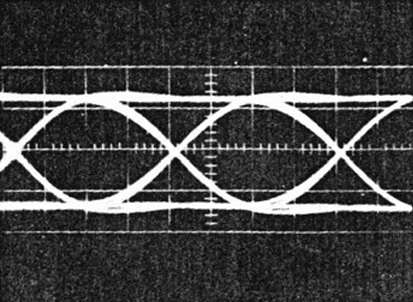
\includegraphics[scale = 0.8]{Esempio di diagramma ad occhio.PNG}
\end{figure} 

Dal punto di vista concettuale, il diagramma ad occhio si ottiene generando tutte le possibili sequenze di simboli binari e graficandone sovrapposti gli andamenti a valle del canale distorcente. \newline 

Un esempio di diagramma ad occhio step-by-step: 

\begin{figure}[h]
    \centering
    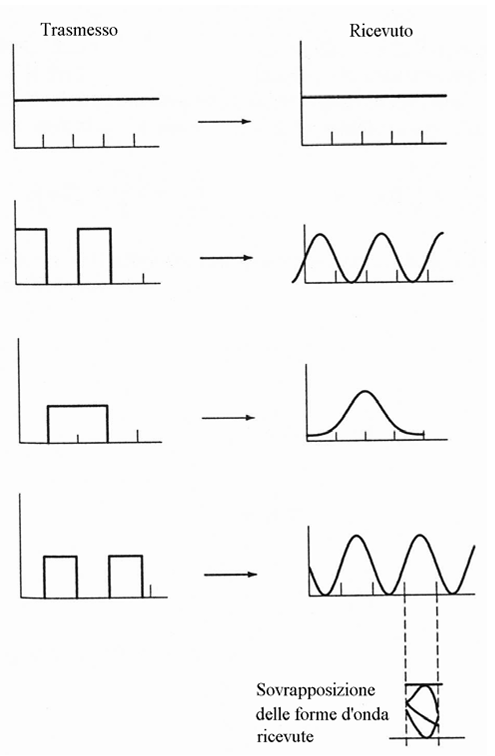
\includegraphics[scale = 0.8]{Diagramma ad occhio step-by-step.PNG}
\end{figure} 

Confrontando diversi diagrammi ad occhio di diverse trasmissioni, possiamo avere i seguenti casi: 

\begin{figure}[h]
    \centering
    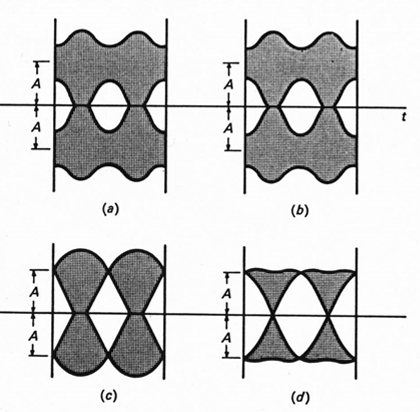
\includegraphics[scale = 0.8]{Diversi diagrammi ad occhio.PNG}
\end{figure} 

\newpage 

L'apertura dell'occhio dà la massima distanza tra i due livelli di decisione. \newline 

Quindi, i casi (c) e (d) sono migliori rispetto ai casi (a) e (b). \newline 

Diagramma ad occhio ideali possono essere ottenuti con una scelta adeguata della funzione di trasferimento del canale, ovvero introducendo una opportuna equalizzazione della funzione di trasferimento di un canale preassegnato. \newline 

\newpage 

\section{Sintesi di un filtro per annullare l'ISI} 

Idealmente, è possibile annullare l'ISI; nella realtà, si cercherà di diminuirlo di tanto. \newline 
Inoltre, l'annullamento non è sempre conseguibile.\newline 

In particolare se la banda B del canale è minore della metà della frequenza di simbolo del segnale numerico, 
in formule: 

{
    \Large 
    \begin{equation}
        B < \frac{F_s}{2} = \frac{1}{2 T_s}    
    \end{equation}
} 

l'obbiettivo dell'annullamento dell'interferenza di intersimbolo non potrà essere, in alcun modo, conseguito. \newline 

Per una data frequenza di simbolo, caratteristica della trasmissione, esiste una larghezzza di banda minima per la banda del canale, al di sotto della quale l'ISI non può essere compensata. \newline 

Dualmente, un sistema caratterizzato da una banda B, se necessario opportunamente equalizzato, può annullare l'interferenza intersimbolica di sistemi con frequenza di simbolo al più uguale a 2B, ma non maggiore. \newline 

Ad esempio, se $B = 1 MHz$, non si può annullare l'ISI di un sistema con frequenza di simbolo $F_s > 2 Mbit/s$. \newline 

Quindi, ponendo $B \geq \frac{F_s}{2}$, possiamo ora fornire alcuni esempi di funzioni di trasferimento in grado di annullare l'interferenza intersimbolica. \newline 

La funzione $H(\omega)$, rappresenta la funzione di traferimento della cascata di reti 2-porte: 

\begin{figure}[h]
    \centering
    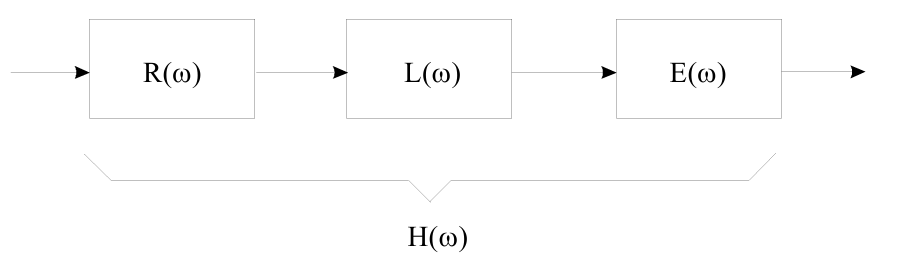
\includegraphics[scale = 0.8]{Cascata reti 2-porte.PNG}
\end{figure} 

Analizzando la cascata di 2-porte, abbiamo che: 
\begin{itemize}
    \item la rete di formazione degli impulsi $R(\omega)$ 
    \item la funzione di trasferimento del mezzo trasmissivo $L(\omega)$ 
    \item la funzione equalizzatrice in ricezione $E(\omega)$
\end{itemize}

Quindi: 

{
    \Large 
    \begin{equation}
        H(\omega) = R(\omega)L(\omega)E(\omega)
    \end{equation}
}

La rete di formazione degli impulsi, in particolare, trasforma una sequenza di Delta di Dirac in ingresso (cui è associata, in senso stretto, l'informazione) 
in una sequenza di impulsi di durata finita: 

\begin{figure}[h]
    \centering
    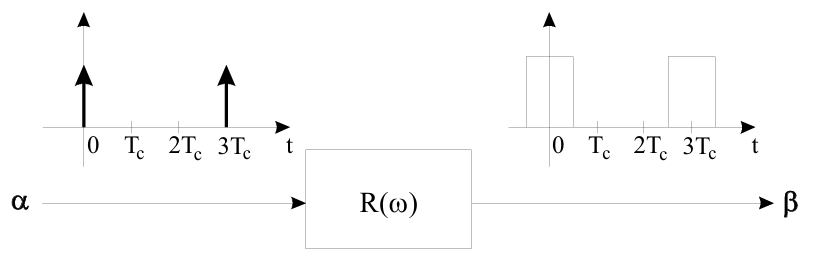
\includegraphics[scale = 0.8]{Rete forazione degli impulsi.PNG}
\end{figure} 

\newpage 

L'informazione trasmessa è chiaramente già contenuta nella successione di Delta di Dirac, ma tale successione non è un segnale fisico (in quanto un impulso matematico ideale non può essere ottenuto in pratica), 
mentre tale risulta la successione di impulsi rettangolari. \newline 

Una prima importante classe di funzioni in grado di annullare l'interferenza di intersimbolo è quella che va sotto il nome di "funzione di trasferimento a coseno rialzato". \newline 

L'espressione analitica di $H(\omega)$ per questa classe di funzioni è la seguente: 

{
    \Large 
    \begin{equation}
        H(\omega) 
        = 
        \begin{cases}
            H_o \text{ per } \abs{\omega} \leq \pi \frac{1 - b}{T_s} \\ 
            \frac{H_o}{2}[1 - \sin(\frac{\abs{\omega} T_s - \pi}{2b})] \text{ per } \pi \frac{1 - b}{T_s} \leq \abs{\omega} \leq \pi \frac{1 + b}{T_s} \\ 
            0 \text{ per } \abs{\omega} \geq \pi \frac{1 - b}{T_s}
        \end{cases}
    \end{equation}
}

dove $H_o$ è una costate reale, mentre b è detto "fattore di roll-off" e varia tra 0 e 1. \newline 

Dal punto di vista grafico e al variare di b, $H(\omega)$ sarà: 

\begin{figure}[h]
    \centering
    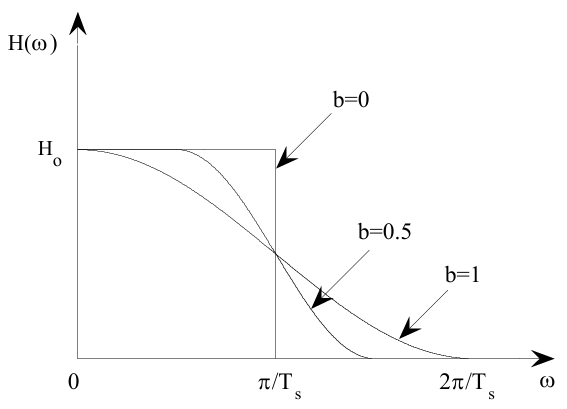
\includegraphics[scale = 0.8]{Funzione di trasferimento a coseno rialzato.PNG}
\end{figure}

La largehezza di banda, espressa in Hz, della funzione di trasferimento a coseno rialzato, vale: 

{
    \Large 
    \begin{equation}
        \begin{split}
            B 
            &= 
            \frac{1}{2 \pi}
            (\pi \frac{1 + b}{T_s}) 
            \\
            &= 
            \frac{1 + b}{2 T_s}
        \end{split}
    \end{equation}
}

Il valore minimo di B è quando $b=0$, che, appunto, è pari a $\frac{1}{2T_s}$. \newline 

Ciò conferma le precedenti considerazioni sulla banda minima in grado di annullare l'ISI e, dall'altra, 
evidenzia che, se l'obbiettivo è quello di minimizzare l'occupazione spettrale, la scelta $b=0$ è la più conveniente. \newline 

Ma, $H(\omega)$ con $b=0$ è impossibile da realizzare con componenti fisici reali (si tratterebbe di un filtro passa-basso ideale), 
mentre la funzione con $b=1$ presenta una transizione più graduale, quindi sarà realizzabile in modo relativamente semplice ed efficiente. \newline 

Inoltre il valore b ottimo dipende non solo da quello che accade nel dominio di $\omega$, 
bensì anche quello che succede nel dominio del tempo. \newline 

Anti-trasformando $H(\omega)$, avremo: 

{
    \Large 
    \begin{equation}
    h(t) 
    = 
    H_o 
    \frac{1}{T_s} 
    \frac{\sin(\frac{\pi}{T_s} t)}{\frac{\pi}{T_s} t}
    \frac{\cos(\frac{\pi}{T_s}) bt}{1 - \frac{4}{T_s ^{2} }b^{2} t^{2}}         
    \end{equation}
}

\begin{figure}[h]
    \centering
    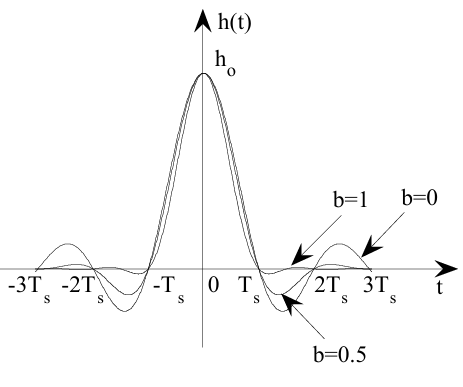
\includegraphics[scale = 0.8]{Anti-trasformata della funzione coseno rialzato.PNG}
\end{figure}

h(t) ha il significato di risposta impulsiva. \newline 

Dalla figura, notiamo che: 

{
    \Large 
    \begin{equation}
        \begin{cases}
            h(0) = h_o \\ 
            h(k T_s) = 0 \text{ per } k = \pm 1, \pm 2, ...
        \end{cases}
    \end{equation}
}

Da queste equazioni, notiamo che, in $t=0$ si annulla l'ISI, e negli altri istanti k non distorce la funzione di ingressi. \newline 

Inoltre, osservando la figura, notiamo che, all'aumentare di b, le code della h(t) risultano maggiormente confinate introrno all'asse dei tempi. \newline 

Quindi, tipicamente, si sceglie un b compreso tra 0.6 e 0.8. \newline 

Inoltre, possiamo notare che la famiglia delle funzioni a coseno rialzato verifica la seguente proprietà: 

{
    \Large 
    \begin{equation}
        \begin{split}
            H_o (\omega_o) 
            &= 
            \sum_{n = -\infty}^{\infty}
            H (\omega_o + n \frac{2 \pi}{T_s})
            \\ 
            &= 
            T_s h_o 
            \text{ per }
            -\frac{\pi}{T_s} \leq \omega_o \leq \frac{\pi}{T_s} 
        \end{split}
    \end{equation}
}

In altre parole, considerata una generica pulsazione $\omega_o$ nell'intervallo $[- \frac{\pi}{T_s}, \frac{\pi}{T_s}]$
la funzione $H_o (\omega_o)$ che si ottiene sommando i valori assunti dalla $H(\omega)$ in $\omega_o$ ed in punti che distano da $\omega_o$ per multipli interi 
di $\frac{2 \pi}{T_s}$ è costante.\newline 

Questa proprietà è nota come criterio di Nyquist, è di validità generale e consente di definire una famiglia di funzioni, 
appunto note come funzioni della classe di Nyquist, tutte in grado di annullare l'interferenza intersimbolica. \newline 

Ritornando a $H(\omega)$, $E(\omega)$ è la rete equilizzatrice in ricezione. \newline 

Una volta scelto il mezzo trasmissivo $L(\omega)$ è assegnata; ad esempio, nel caso di un cavo coassiale, sotto l'ipotesi di piccole perdite, si può scrivere: 

{
    \Large 
    \begin{equation}
        L(\omega) = \exp [- \sqrt{\frac{\omega}{\omega_o}} (1+ \jmath) -\jmath \omega t_c]
    \end{equation}
}

dove $\omega_o$ è una pulsazione caratteristica, mentre $t_c$ è il tempo di propagazione delle onde elettromagnetiche nel mezzo. \newline 

Il prodotto $R(\omega) \cdot L (\omega)$ appartiene alla classe di Nyquist; 
in generale, è quindi necessario introdurre l'opportuna correzione attraverso $E(\omega)$. \newline 

Graficamente: 

\begin{figure}[h]
    \centering
    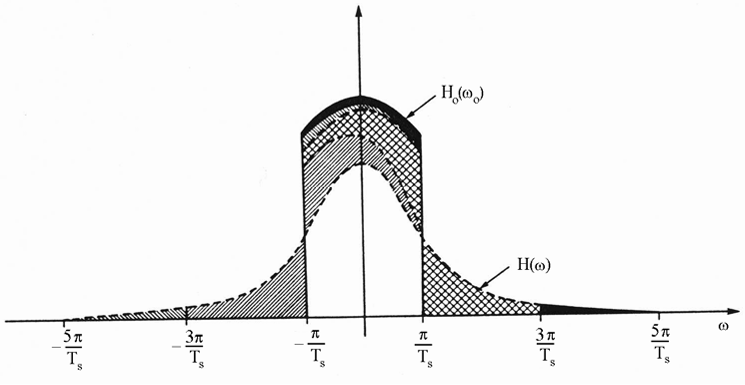
\includegraphics[scale = 0.8]{Spettro della cascata delle reti 2-porte.PNG}
\end{figure}


Chiaramente deve essere: 

{
    \Large 
    \begin{equation}
        E(\omega) R(\omega) = \frac{H(\omega)}{L(\omega)}
    \end{equation}
}

Una soluzione molto frequente è quella di porre: 

{
    \Large 
    \begin{equation}
        \abs{E(\omega)} = \abs{R(\omega)} = \sqrt{\frac{\abs{H(\omega)}}{\abs{L(\omega)}}}
    \end{equation}
}

Scegliendo arbitrariamente la fase di $E(\omega)$. \newline 

Se il rapporto $\frac{H(\omega)}{L(\omega)}$ è reale, si può porre semplicemente: 

{
    \Large 
    \begin{equation}
        E(\omega) = R^{*} (\omega)
    \end{equation}
}

\newpage 
. 
\newpage 
. 
\newpage